	This section defines the concept of \emph{\pos}\ (originally introduced
        in~\cite{Gerbrandy1997}), based on \nwf\ set theory.
	This section aims to provide the reader with enough information to understand what \posS\ are.
	
	For a more informative introduction the reader is addressed to~\cite{gerbrandy1999bisimulations,Aczel1989-ACZNS-2,barwise1987liar} and to~\cite{DBLP:conf/iclp/Dovier15} for a logic programming point of view on
	\nwf\ sets and their equivalence.
%	Familiarity with set and graph theory is assumed.
	%
	%
	\subsection{\Nwf\ set theory fundamentals}\label{subsec-possibilities:set_th}
	We start by giving some fundamental definitions of \nwf\ set theory.
	First of all a \emph{\wf}\ \emph{set} is described in~\cite{Aczel1989-ACZNS-2} as follows:
	\begin{definition}[\wf\ set]\label{def:wfs}
		Let $E$ be a set, $E^\prime$ one of its elements, $E^{\prime\prime}$ any element of $E^\prime$, and so on. A descent is the sequence of steps from $E$ to $E^\prime$, $E^\prime$ to $E^{\prime\prime}$, etc. $\dots$\ A set is 
		\emph{\wf}\ (or \emph{ordinary}) when it only gives rise to finite descents.
		%; and it is
		%\nwf\ (or extraordinary) when among its descents there are some which are infinite.
	\end{definition}
	%
	\Wf\ set theory states that all the sets in the sense of Definition~\ref{def:wfs} can be represented in the form of graphs, called \emph{pictures}, (as shown in Figure~\ref{fig:von_neu_ord}).
	%
	\begin{figure}
		\centering
		\subfloat[Pictures of von Neumann ordinals where 
		$0=\emptyset$;
		$1=\bra{\emptyset}$;
		$2=\bra{\emptyset, \bra{\emptyset}}$;
		$3=\bra{\emptyset,\bra{\emptyset},\bra{\emptyset,\bra{\emptyset}}}$.]{\scalebox{0.7}{

\tikzset{every picture/.style={line width=0.75pt}} %set default line width to 0.75pt        

\begin{tikzpicture}[x=0.75pt,y=0.75pt,yscale=-0.7,xscale=0.7]
%uncomment if require: \path (0,243); %set diagram left start at 0, and has height of 243

%Straight Lines [id:da42363008311855377] 
\draw    (126.5,47) ;
\draw [shift={(126.5,47)}, rotate = 0] [color={rgb, 255:red, 0; green, 0; blue, 0 }  ][fill={rgb, 255:red, 0; green, 0; blue, 0 }  ][line width=0.75]      (0, 0) circle [x radius= 3.35, y radius= 3.35]   ;

%Straight Lines [id:da9776475110732991] 
\draw    (196.5,47) -- (196.5,111) ;
\draw [shift={(196.5,111)}, rotate = 90] [color={rgb, 255:red, 0; green, 0; blue, 0 }  ][fill={rgb, 255:red, 0; green, 0; blue, 0 }  ][line width=0.75]      (0, 0) circle [x radius= 3.35, y radius= 3.35]   ;
\draw [shift={(196.5,47)}, rotate = 90] [color={rgb, 255:red, 0; green, 0; blue, 0 }  ][fill={rgb, 255:red, 0; green, 0; blue, 0 }  ][line width=0.75]      (0, 0) circle [x radius= 3.35, y radius= 3.35]   ;
%Straight Lines [id:da161306486001776] 
\draw    (300.5,47) -- (274.5,110) ;
\draw [shift={(274.5,110)}, rotate = 112.43] [color={rgb, 255:red, 0; green, 0; blue, 0 }  ][fill={rgb, 255:red, 0; green, 0; blue, 0 }  ][line width=0.75]      (0, 0) circle [x radius= 3.35, y radius= 3.35]   ;
\draw [shift={(300.5,47)}, rotate = 112.43] [color={rgb, 255:red, 0; green, 0; blue, 0 }  ][fill={rgb, 255:red, 0; green, 0; blue, 0 }  ][line width=0.75]      (0, 0) circle [x radius= 3.35, y radius= 3.35]   ;
%Straight Lines [id:da12831723727076116] 
\draw    (300.5,47) -- (323.5,110) ;
\draw [shift={(323.5,110)}, rotate = 69.94] [color={rgb, 255:red, 0; green, 0; blue, 0 }  ][fill={rgb, 255:red, 0; green, 0; blue, 0 }  ][line width=0.75]      (0, 0) circle [x radius= 3.35, y radius= 3.35]   ;
\draw [shift={(300.5,47)}, rotate = 69.94] [color={rgb, 255:red, 0; green, 0; blue, 0 }  ][fill={rgb, 255:red, 0; green, 0; blue, 0 }  ][line width=0.75]      (0, 0) circle [x radius= 3.35, y radius= 3.35]   ;
%Straight Lines [id:da5112115278285075] 
\draw    (323.5,110) -- (323.5,172) ;
\draw [shift={(323.5,172)}, rotate = 90] [color={rgb, 255:red, 0; green, 0; blue, 0 }  ][fill={rgb, 255:red, 0; green, 0; blue, 0 }  ][line width=0.75]      (0, 0) circle [x radius= 3.35, y radius= 3.35]   ;
\draw [shift={(323.5,110)}, rotate = 90] [color={rgb, 255:red, 0; green, 0; blue, 0 }  ][fill={rgb, 255:red, 0; green, 0; blue, 0 }  ][line width=0.75]      (0, 0) circle [x radius= 3.35, y radius= 3.35]   ;
%Straight Lines [id:da8536132167008245] 
\draw    (426.5,46) -- (400.5,109) ;
\draw [shift={(400.5,109)}, rotate = 112.43] [color={rgb, 255:red, 0; green, 0; blue, 0 }  ][fill={rgb, 255:red, 0; green, 0; blue, 0 }  ][line width=0.75]      (0, 0) circle [x radius= 3.35, y radius= 3.35]   ;
\draw [shift={(426.5,46)}, rotate = 112.43] [color={rgb, 255:red, 0; green, 0; blue, 0 }  ][fill={rgb, 255:red, 0; green, 0; blue, 0 }  ][line width=0.75]      (0, 0) circle [x radius= 3.35, y radius= 3.35]   ;
%Straight Lines [id:da7449065643500326] 
\draw    (426.5,46) -- (449.5,109) ;
\draw [shift={(449.5,109)}, rotate = 69.94] [color={rgb, 255:red, 0; green, 0; blue, 0 }  ][fill={rgb, 255:red, 0; green, 0; blue, 0 }  ][line width=0.75]      (0, 0) circle [x radius= 3.35, y radius= 3.35]   ;
\draw [shift={(426.5,46)}, rotate = 69.94] [color={rgb, 255:red, 0; green, 0; blue, 0 }  ][fill={rgb, 255:red, 0; green, 0; blue, 0 }  ][line width=0.75]      (0, 0) circle [x radius= 3.35, y radius= 3.35]   ;
%Straight Lines [id:da07257306396931185] 
\draw    (449.5,109) -- (449.5,171) ;
\draw [shift={(449.5,171)}, rotate = 90] [color={rgb, 255:red, 0; green, 0; blue, 0 }  ][fill={rgb, 255:red, 0; green, 0; blue, 0 }  ][line width=0.75]      (0, 0) circle [x radius= 3.35, y radius= 3.35]   ;
\draw [shift={(449.5,109)}, rotate = 90] [color={rgb, 255:red, 0; green, 0; blue, 0 }  ][fill={rgb, 255:red, 0; green, 0; blue, 0 }  ][line width=0.75]      (0, 0) circle [x radius= 3.35, y radius= 3.35]   ;
%Straight Lines [id:da021322635576809246] 
\draw    (426.5,46) -- (494.5,110) ;
\draw [shift={(494.5,110)}, rotate = 43.26] [color={rgb, 255:red, 0; green, 0; blue, 0 }  ][fill={rgb, 255:red, 0; green, 0; blue, 0 }  ][line width=0.75]      (0, 0) circle [x radius= 3.35, y radius= 3.35]   ;
\draw [shift={(426.5,46)}, rotate = 43.26] [color={rgb, 255:red, 0; green, 0; blue, 0 }  ][fill={rgb, 255:red, 0; green, 0; blue, 0 }  ][line width=0.75]      (0, 0) circle [x radius= 3.35, y radius= 3.35]   ;
%Straight Lines [id:da9755353003788908] 
\draw    (494.5,110) -- (468.5,173) ;
\draw [shift={(468.5,173)}, rotate = 112.43] [color={rgb, 255:red, 0; green, 0; blue, 0 }  ][fill={rgb, 255:red, 0; green, 0; blue, 0 }  ][line width=0.75]      (0, 0) circle [x radius= 3.35, y radius= 3.35]   ;
\draw [shift={(494.5,110)}, rotate = 112.43] [color={rgb, 255:red, 0; green, 0; blue, 0 }  ][fill={rgb, 255:red, 0; green, 0; blue, 0 }  ][line width=0.75]      (0, 0) circle [x radius= 3.35, y radius= 3.35]   ;
%Straight Lines [id:da12250203413215166] 
\draw    (494.5,110) -- (517.5,173) ;
\draw [shift={(517.5,173)}, rotate = 69.94] [color={rgb, 255:red, 0; green, 0; blue, 0 }  ][fill={rgb, 255:red, 0; green, 0; blue, 0 }  ][line width=0.75]      (0, 0) circle [x radius= 3.35, y radius= 3.35]   ;
\draw [shift={(494.5,110)}, rotate = 69.94] [color={rgb, 255:red, 0; green, 0; blue, 0 }  ][fill={rgb, 255:red, 0; green, 0; blue, 0 }  ][line width=0.75]      (0, 0) circle [x radius= 3.35, y radius= 3.35]   ;
%Straight Lines [id:da4220154805716767] 
\draw    (517.5,173) -- (517.5,235) ;
\draw [shift={(517.5,235)}, rotate = 90] [color={rgb, 255:red, 0; green, 0; blue, 0 }  ][fill={rgb, 255:red, 0; green, 0; blue, 0 }  ][line width=0.75]      (0, 0) circle [x radius= 3.35, y radius= 3.35]   ;
\draw [shift={(517.5,173)}, rotate = 90] [color={rgb, 255:red, 0; green, 0; blue, 0 }  ][fill={rgb, 255:red, 0; green, 0; blue, 0 }  ][line width=0.75]      (0, 0) circle [x radius= 3.35, y radius= 3.35]   ;
%Straight Lines [id:da34828451096237323] 
\draw    (438,77.5) -- (441.87,89.1) ;
\draw [shift={(442.5,91)}, rotate = 251.57] [fill={rgb, 255:red, 0; green, 0; blue, 0 }  ][line width=0.75]  [draw opacity=0] (8.93,-4.29) -- (0,0) -- (8.93,4.29) -- cycle    ;

%Straight Lines [id:da847083601142183] 
\draw    (413.5,77.5) -- (410.21,86.13) ;
\draw [shift={(409.5,88)}, rotate = 290.85] [fill={rgb, 255:red, 0; green, 0; blue, 0 }  ][line width=0.75]  [draw opacity=0] (8.93,-4.29) -- (0,0) -- (8.93,4.29) -- cycle    ;

%Straight Lines [id:da8305126214716252] 
\draw    (449.5,137) -- (449.5,145) ;
\draw [shift={(449.5,147)}, rotate = 270] [fill={rgb, 255:red, 0; green, 0; blue, 0 }  ][line width=0.75]  [draw opacity=0] (8.93,-4.29) -- (0,0) -- (8.93,4.29) -- cycle    ;

%Straight Lines [id:da0020619886975261625] 
\draw    (506,141.5) -- (509.77,151.14) ;
\draw [shift={(510.5,153)}, rotate = 248.63] [fill={rgb, 255:red, 0; green, 0; blue, 0 }  ][line width=0.75]  [draw opacity=0] (8.93,-4.29) -- (0,0) -- (8.93,4.29) -- cycle    ;

%Straight Lines [id:da8008262780720901] 
\draw    (517.5,204) -- (517.5,212) ;
\draw [shift={(517.5,214)}, rotate = 270] [fill={rgb, 255:red, 0; green, 0; blue, 0 }  ][line width=0.75]  [draw opacity=0] (8.93,-4.29) -- (0,0) -- (8.93,4.29) -- cycle    ;

%Straight Lines [id:da5166796275526594] 
\draw    (481.5,141.5) -- (477.3,151.17) ;
\draw [shift={(476.5,153)}, rotate = 293.5] [fill={rgb, 255:red, 0; green, 0; blue, 0 }  ][line width=0.75]  [draw opacity=0] (8.93,-4.29) -- (0,0) -- (8.93,4.29) -- cycle    ;

%Straight Lines [id:da2483045453323448] 
\draw    (460.5,78) -- (472.03,88.64) ;
\draw [shift={(473.5,90)}, rotate = 222.71] [fill={rgb, 255:red, 0; green, 0; blue, 0 }  ][line width=0.75]  [draw opacity=0] (8.93,-4.29) -- (0,0) -- (8.93,4.29) -- cycle    ;


%Straight Lines [id:da5301987015108148] 
\draw    (196.5,69) -- (196.5,77) ;
\draw [shift={(196.5,79)}, rotate = 270] [fill={rgb, 255:red, 0; green, 0; blue, 0 }  ][line width=0.75]  [draw opacity=0] (8.93,-4.29) -- (0,0) -- (8.93,4.29) -- cycle    ;

%Straight Lines [id:da9808201842892292] 
\draw    (287.5,78.5) -- (282.22,92.13) ;
\draw [shift={(281.5,94)}, rotate = 291.15999999999997] [fill={rgb, 255:red, 0; green, 0; blue, 0 }  ][line width=0.75]  [draw opacity=0] (8.93,-4.29) -- (0,0) -- (8.93,4.29) -- cycle    ;

%Straight Lines [id:da9287523922345057] 
\draw    (313,82.5) -- (316.82,93.12) ;
\draw [shift={(317.5,95)}, rotate = 250.2] [fill={rgb, 255:red, 0; green, 0; blue, 0 }  ][line width=0.75]  [draw opacity=0] (8.93,-4.29) -- (0,0) -- (8.93,4.29) -- cycle    ;

%Straight Lines [id:da02578212493217935] 
\draw    (323.5,141) -- (323.5,149) ;
\draw [shift={(323.5,151)}, rotate = 270] [fill={rgb, 255:red, 0; green, 0; blue, 0 }  ][line width=0.75]  [draw opacity=0] (8.93,-4.29) -- (0,0) -- (8.93,4.29) -- cycle    ;


% Text Node
\draw (130,22) node   {$0$};
% Text Node
\draw (197,22) node   {$1$};
% Text Node
\draw (300,22) node   {$2$};
% Text Node
\draw (427,22) node   {$3$};


\draw (60,22) node   {};
\draw (585,22) node   {};


\end{tikzpicture}

}\label{subfig-1:von_neu_ord}}
		\hfill
		\subfloat[Alternative Pictures of von Neumann ordinals 2 and 3.]{\scalebox{0.8}{\tikzset{every picture/.style={line width=0.75pt}} %set default line width to 0.75pt        

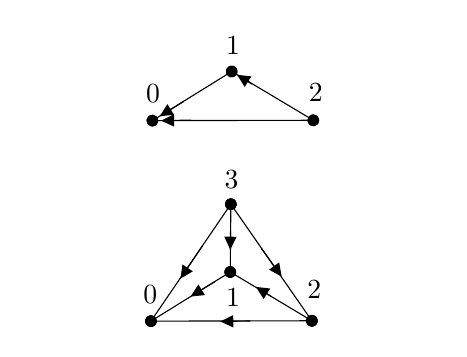
\begin{tikzpicture}[x=0.75pt,y=0.75pt,yscale=-0.7,xscale=0.7]\tikzset{every picture/.style={line width=0.75pt}}

%Straight Lines [id:da31341595090350494] 
\draw    (149.25,245.25) -- (38.5,245.5) ;
\draw [shift={(38.5,245.5)}, rotate = 179.87] [color={rgb, 255:red, 0; green, 0; blue, 0 }  ][fill={rgb, 255:red, 0; green, 0; blue, 0 }  ][line width=0.75]      (0, 0) circle [x radius= 3.35, y radius= 3.35]   ;
\draw [shift={(149.25,245.25)}, rotate = 179.87] [color={rgb, 255:red, 0; green, 0; blue, 0 }  ][fill={rgb, 255:red, 0; green, 0; blue, 0 }  ][line width=0.75]      (0, 0) circle [x radius= 3.35, y radius= 3.35]   ;
%Straight Lines [id:da9609296906616727] 
\draw    (106.88,245.38) -- (88.25,245.71) ;
\draw [shift={(86.25,245.75)}, rotate = 358.96000000000004] [fill={rgb, 255:red, 0; green, 0; blue, 0 }  ][line width=0.75]  [draw opacity=0] (8.93,-4.29) -- (0,0) -- (8.93,4.29) -- cycle    ;

%Straight Lines [id:da252345846123192] 
\draw    (93.5,165) -- (38.5,245.5) ;
\draw [shift={(38.5,245.5)}, rotate = 124.34] [color={rgb, 255:red, 0; green, 0; blue, 0 }  ][fill={rgb, 255:red, 0; green, 0; blue, 0 }  ][line width=0.75]      (0, 0) circle [x radius= 3.35, y radius= 3.35]   ;
\draw [shift={(93.5,165)}, rotate = 124.34] [color={rgb, 255:red, 0; green, 0; blue, 0 }  ][fill={rgb, 255:red, 0; green, 0; blue, 0 }  ][line width=0.75]      (0, 0) circle [x radius= 3.35, y radius= 3.35]   ;
%Straight Lines [id:da11171836378352906] 
\draw    (73.96,193.6) -- (59.88,214.61) ;
\draw [shift={(58.77,216.27)}, rotate = 303.83] [fill={rgb, 255:red, 0; green, 0; blue, 0 }  ][line width=0.75]  [draw opacity=0] (8.93,-4.29) -- (0,0) -- (8.93,4.29) -- cycle    ;

%Straight Lines [id:da9411846809932387] 
\draw    (149.25,245.25) -- (93.5,165) ;
\draw [shift={(93.5,165)}, rotate = 235.21] [color={rgb, 255:red, 0; green, 0; blue, 0 }  ][fill={rgb, 255:red, 0; green, 0; blue, 0 }  ][line width=0.75]      (0, 0) circle [x radius= 3.35, y radius= 3.35]   ;
\draw [shift={(149.25,245.25)}, rotate = 235.21] [color={rgb, 255:red, 0; green, 0; blue, 0 }  ][fill={rgb, 255:red, 0; green, 0; blue, 0 }  ][line width=0.75]      (0, 0) circle [x radius= 3.35, y radius= 3.35]   ;
%Straight Lines [id:da6467035917598132] 
\draw    (114.71,195.71) -- (127.31,213.19) ;
\draw [shift={(128.48,214.81)}, rotate = 234.21] [fill={rgb, 255:red, 0; green, 0; blue, 0 }  ][line width=0.75]  [draw opacity=0] (8.93,-4.29) -- (0,0) -- (8.93,4.29) -- cycle    ;

%Straight Lines [id:da05960945318721844] 
\draw    (93.5,165) -- (93.08,211.67) ;
\draw [shift={(93.08,211.67)}, rotate = 90.51] [color={rgb, 255:red, 0; green, 0; blue, 0 }  ][fill={rgb, 255:red, 0; green, 0; blue, 0 }  ][line width=0.75]      (0, 0) circle [x radius= 3.35, y radius= 3.35]   ;
\draw [shift={(93.5,165)}, rotate = 90.51] [color={rgb, 255:red, 0; green, 0; blue, 0 }  ][fill={rgb, 255:red, 0; green, 0; blue, 0 }  ][line width=0.75]      (0, 0) circle [x radius= 3.35, y radius= 3.35]   ;
%Straight Lines [id:da18779983245814547] 
\draw    (93.08,211.67) -- (38.5,245.5) ;
\draw [shift={(38.5,245.5)}, rotate = 148.21] [color={rgb, 255:red, 0; green, 0; blue, 0 }  ][fill={rgb, 255:red, 0; green, 0; blue, 0 }  ][line width=0.75]      (0, 0) circle [x radius= 3.35, y radius= 3.35]   ;
\draw [shift={(93.08,211.67)}, rotate = 148.21] [color={rgb, 255:red, 0; green, 0; blue, 0 }  ][fill={rgb, 255:red, 0; green, 0; blue, 0 }  ][line width=0.75]      (0, 0) circle [x radius= 3.35, y radius= 3.35]   ;
%Straight Lines [id:da9874513451972009] 
\draw    (93.08,211.67) -- (149.25,245.25) ;
\draw [shift={(149.25,245.25)}, rotate = 30.88] [color={rgb, 255:red, 0; green, 0; blue, 0 }  ][fill={rgb, 255:red, 0; green, 0; blue, 0 }  ][line width=0.75]      (0, 0) circle [x radius= 3.35, y radius= 3.35]   ;
\draw [shift={(93.08,211.67)}, rotate = 30.88] [color={rgb, 255:red, 0; green, 0; blue, 0 }  ][fill={rgb, 255:red, 0; green, 0; blue, 0 }  ][line width=0.75]      (0, 0) circle [x radius= 3.35, y radius= 3.35]   ;
%Straight Lines [id:da21738250880340737] 
\draw    (82.42,218.33) -- (67.49,227.53) ;
\draw [shift={(65.79,228.58)}, rotate = 328.34000000000003] [fill={rgb, 255:red, 0; green, 0; blue, 0 }  ][line width=0.75]  [draw opacity=0] (8.93,-4.29) -- (0,0) -- (8.93,4.29) -- cycle    ;

%Straight Lines [id:da502837847841804] 
\draw    (93.29,183.33) -- (93.13,194.32) ;
\draw [shift={(93.1,196.32)}, rotate = 270.83] [fill={rgb, 255:red, 0; green, 0; blue, 0 }  ][line width=0.75]  [draw opacity=0] (8.93,-4.29) -- (0,0) -- (8.93,4.29) -- cycle    ;

%Straight Lines [id:da38006772268977085] 
\draw    (121.17,228.46) -- (112.46,223) ;
\draw [shift={(110.76,221.94)}, rotate = 392.05] [fill={rgb, 255:red, 0; green, 0; blue, 0 }  ][line width=0.75]  [draw opacity=0] (8.93,-4.29) -- (0,0) -- (8.93,4.29) -- cycle    ;

%Straight Lines [id:da09733860617343582] 
\draw    (150.25,107.25) -- (39.5,107.5) ;
\draw [shift={(39.5,107.5)}, rotate = 179.87] [color={rgb, 255:red, 0; green, 0; blue, 0 }  ][fill={rgb, 255:red, 0; green, 0; blue, 0 }  ][line width=0.75]      (0, 0) circle [x radius= 3.35, y radius= 3.35]   ;
\draw [shift={(150.25,107.25)}, rotate = 179.87] [color={rgb, 255:red, 0; green, 0; blue, 0 }  ][fill={rgb, 255:red, 0; green, 0; blue, 0 }  ][line width=0.75]      (0, 0) circle [x radius= 3.35, y radius= 3.35]   ;
%Straight Lines [id:da9907229664589221] 
\draw    (66.13,107.13) -- (47.5,107.46) ;
\draw [shift={(45.5,107.5)}, rotate = 358.96000000000004] [fill={rgb, 255:red, 0; green, 0; blue, 0 }  ][line width=0.75]  [draw opacity=0] (8.93,-4.29) -- (0,0) -- (8.93,4.29) -- cycle    ;

%Straight Lines [id:da8984506786350759] 
\draw    (94.08,73.67) -- (39.5,107.5) ;
\draw [shift={(39.5,107.5)}, rotate = 148.21] [color={rgb, 255:red, 0; green, 0; blue, 0 }  ][fill={rgb, 255:red, 0; green, 0; blue, 0 }  ][line width=0.75]      (0, 0) circle [x radius= 3.35, y radius= 3.35]   ;
\draw [shift={(94.08,73.67)}, rotate = 148.21] [color={rgb, 255:red, 0; green, 0; blue, 0 }  ][fill={rgb, 255:red, 0; green, 0; blue, 0 }  ][line width=0.75]      (0, 0) circle [x radius= 3.35, y radius= 3.35]   ;
%Straight Lines [id:da13062093153249577] 
\draw    (94.08,73.67) -- (150.25,107.25) ;
\draw [shift={(150.25,107.25)}, rotate = 30.88] [color={rgb, 255:red, 0; green, 0; blue, 0 }  ][fill={rgb, 255:red, 0; green, 0; blue, 0 }  ][line width=0.75]      (0, 0) circle [x radius= 3.35, y radius= 3.35]   ;
\draw [shift={(94.08,73.67)}, rotate = 30.88] [color={rgb, 255:red, 0; green, 0; blue, 0 }  ][fill={rgb, 255:red, 0; green, 0; blue, 0 }  ][line width=0.75]      (0, 0) circle [x radius= 3.35, y radius= 3.35]   ;
%Straight Lines [id:da9384075142317254] 
\draw    (61.13,94.25) -- (46.2,103.45) ;
\draw [shift={(44.5,104.5)}, rotate = 328.34000000000003] [fill={rgb, 255:red, 0; green, 0; blue, 0 }  ][line width=0.75]  [draw opacity=0] (8.93,-4.29) -- (0,0) -- (8.93,4.29) -- cycle    ;

%Straight Lines [id:da2991130569955017] 
\draw    (108.17,82.46) -- (99.46,77) ;
\draw [shift={(97.76,75.94)}, rotate = 392.05] [fill={rgb, 255:red, 0; green, 0; blue, 0 }  ][line width=0.75]  [draw opacity=0] (8.93,-4.29) -- (0,0) -- (8.93,4.29) -- cycle    ;


% Text Node
\draw (94,148) node   {$3$};
% Text Node
\draw (152,88) node   {$2$};
% Text Node
\draw (95,56) node   {$1$};
% Text Node
\draw (151,224) node   {$2$};
% Text Node
\draw (95,229) node   {$1$};
% Text Node
\draw (38,227) node   {$0$};
% Text Node
\draw (40,89) node   {$0$};


\draw (-40,89) node   {};
\draw (230,56) node   {};

\end{tikzpicture}
}\label{subfig-2:von_neu_ord}}
		\caption{\Wf\ sets represented through graphs~\cite{Aczel1989-ACZNS-2}.}
		\label{fig:von_neu_ord}
	\end{figure}
	To formalize this concept of \textquoteleft picture of a set' however it is necessary to introduce the concept of \emph{decoration}:
	%
	\begin{definition} [decoration and picture]
		\begin{itemize}
			\item A \emph{decoration} of a graph \graphVE{V}{E}\ is a function $\delta$ that assigns to each node $\defemph{n} \in V$\ a set $\delta_\defemph{n}$ in such a way that the elements of $\delta_\defemph{n}$ are exactly the sets assigned to successors of \defemph{n}, \ie $\delta_\defemph{n} = \{\delta_\defemph{n^{\prime}} \mid (\defemph{n},\defemph{n}^\prime) \in E\}$.
		
			\item If $\delta$ is a decoration of a pointed graph $(\graphG, \defemph{n})$, then $(\graphG, \defemph{n})$ is a \emph{picture} of the set $\delta_\defemph{n}$.
		\end{itemize}
	\end{definition}
	%
	Moreover, in well-founded set theory, it holds the Mostovski's lemma: \textquotedblleft each \wf\ graph\footnote{A \wf\ graph is a graph that doesn't contain an infinite path $\defemph{n} \rightarrow \defemph{n}^{\prime} \rightarrow \defemph{n}^{\prime\prime} \rightarrow \dots$ of successors.} is a picture of exactly one set".

	
	On the other hand in~\cite{Aczel1989-ACZNS-2} a \emph{\nwf}, or \emph{extraordinary set} in the sense of Mirimanoff, is a set that respects Definition~\ref{def:nwfs}.
	\begin{definition}[\nwf\ set]\label{def:nwfs}
		A set is \emph{\nwf}\ (or \emph{extraordinary}) when among its descents there are some which are infinite.
	\end{definition}
	%
	In fact, when the \textbf{Foundation Axiom}\footnote{Expressed in~\cite{gerbrandy1999bisimulations} as \textquotedblleft Only \wf\ graphs have decorations".} is substituted by the \textbf{Anti-Foundation Axiom} (\textbf{AFA}), expressed by Aczel in~\cite{Aczel1989-ACZNS-2} as \textquotedblleft \textit{Every graph has a unique decoration}", the following consequences become true:
	\begin{itemize}
		%\item Every pointed graph is a picture of a unique set;
			\item Every graph is a picture of exactly one set (\textbf{AFA} as is formulated in~\cite{gerbrandy1999bisimulations});
		\item \nwf\ sets exist given that a \nwf\ pointed graph has to be a picture of a \nwf\ set.
		%\item every graph is a picture of exactly one set (\textbf{AFA} as is formulated in~\cite{gerbrandy1999bisimulations}).
	\end{itemize}
	%
	\begin{figure}
		\centering
		\subfloat[Standard picture $\Omega$.]{\scalebox{0.6}{\input{img/omega}}\label{subfig-omega_nwf:1}}
		\hfill
		\subfloat[Unfolding of the picture of $\Omega$.]{\scalebox{1}{

\tikzset{every picture/.style={line width=0.75pt}} %set default line width to 0.75pt        

\begin{tikzpicture}[x=0.75pt,y=0.75pt,yscale=-1,xscale=1]
%uncomment if require: \path (0,300); %set diagram left start at 0, and has height of 300

%Straight Lines [id:da6276790682079358] 
\draw    (100.6,110) -- (140.85,110) ;


%Flowchart: Connector [id:dp10712755168097865] 
\draw  [fill={rgb, 255:red, 0; green, 0; blue, 0 }  ,fill opacity=1 ] (103,110) .. controls (103,111.33) and (101.93,112.4) .. (100.6,112.4) .. controls (99.27,112.4) and (98.2,111.33) .. (98.2,110) .. controls (98.2,108.67) and (99.27,107.6) .. (100.6,107.6) .. controls (101.93,107.6) and (103,108.67) .. (103,110) -- cycle ;
%Straight Lines [id:da8191358904406301] 
\draw    (139.8,110.2) -- (180.05,110.2) ;


%Flowchart: Connector [id:dp9628511983929124] 
\draw  [fill={rgb, 255:red, 0; green, 0; blue, 0 }  ,fill opacity=1 ] (142.2,110.2) .. controls (142.2,111.53) and (141.13,112.6) .. (139.8,112.6) .. controls (138.47,112.6) and (137.4,111.53) .. (137.4,110.2) .. controls (137.4,108.87) and (138.47,107.8) .. (139.8,107.8) .. controls (141.13,107.8) and (142.2,108.87) .. (142.2,110.2) -- cycle ;
%Shape: Triangle [id:dp18185199166706778] 
\draw  [fill={rgb, 255:red, 0; green, 0; blue, 0 }  ,fill opacity=1 ] (120.72,110) -- (118,111.21) -- (118,108.79) -- cycle ;
%Shape: Triangle [id:dp11767706980455106] 
\draw  [color={rgb, 255:red, 0; green, 0; blue, 0 }  ,draw opacity=1 ][fill={rgb, 255:red, 0; green, 0; blue, 0 }  ,fill opacity=1 ] (159.92,110.2) -- (157.2,111.41) -- (157.2,108.99) -- cycle ;
%Straight Lines [id:da6334935852876922] 
\draw    (180.1,110) -- (220.35,110) ;


%Flowchart: Connector [id:dp022374442404981654] 
\draw  [fill={rgb, 255:red, 0; green, 0; blue, 0 }  ,fill opacity=1 ] (182.5,110) .. controls (182.5,111.33) and (181.43,112.4) .. (180.1,112.4) .. controls (178.77,112.4) and (177.7,111.33) .. (177.7,110) .. controls (177.7,108.67) and (178.77,107.6) .. (180.1,107.6) .. controls (181.43,107.6) and (182.5,108.67) .. (182.5,110) -- cycle ;
%Flowchart: Connector [id:dp8113410302855639] 
\draw  [fill={rgb, 255:red, 0; green, 0; blue, 0 }  ,fill opacity=1 ] (221.7,110.2) .. controls (221.7,111.53) and (220.63,112.6) .. (219.3,112.6) .. controls (217.97,112.6) and (216.9,111.53) .. (216.9,110.2) .. controls (216.9,108.87) and (217.97,107.8) .. (219.3,107.8) .. controls (220.63,107.8) and (221.7,108.87) .. (221.7,110.2) -- cycle ;
%Shape: Triangle [id:dp5972516863295354] 
\draw  [fill={rgb, 255:red, 0; green, 0; blue, 0 }  ,fill opacity=1 ] (200.22,110) -- (197.5,111.21) -- (197.5,108.79) -- cycle ;
%Straight Lines [id:da9015443131541547] 
\draw  [dash pattern={on 0.84pt off 2.51pt}]  (219.3,110.2) -- (250.15,110.2) ;

\draw (250,140) node   {};
\draw (90,140) node   {};


\end{tikzpicture}

}\label{subfig-omega_nwf:2}}
		\caption{Representation of the \nwf\ set $\Omega = \{\Omega\}$~\cite{Aczel1989-ACZNS-2}.}
		\label{fig:omega_nwf}
	\end{figure}


%We can now reformulate \textbf{AFA} as in~\cite{gerbrandy1999bisimulations} to
%	\subsection{Systems of Equations}
%	\Nwf\ sets, as said in \S~\ref{subsec-possibilities:set_th}, can be represented by \nwf\ graphs.
	In~\cite{Aczel1989-ACZNS-2,gerbrandy1999bisimulations} it is pointed out how \nwf\ sets can also be expressed through systems of equations. 
	This concept will help us to formalize the notion of state in our action language.
	
	A quick example of this representation can be derived by the set $\Omega = \{\Omega\}$ (Figure~\ref{fig:omega_nwf}). We can, in fact, informally define this set by the (singleton) system of equations $%\big\{%
	x = \bra{x}$.
	%
	Systems of equations and their solutions are described more formally as follows in~\cite{gerbrandy1999bisimulations}:
	%
	\begin{definition}[system of equations]
		For each class of atoms\footnote{Objects that are not sets and have no further set-theoretic structure.} $\mathcal{X}$ a \emph{system of equation} in $\mathcal{X}$ is a class
		$\tau$ of equations $\poss{x} = \mathtt{X}$, where $\poss{x} \in \mathcal{X}$ and $\mathtt{X} \subseteq \mathcal{X}$, such that  $\tau$ contains exactly one equation $\poss{x} = \mathtt{X}$ for each $\poss{x} \in \mathcal{X}$. 
		%that for each $\poss{x} \in \mathcal{X}$ includes exactly one equation of the form $\poss{x} = \mathtt{X}$ where $\mathtt{X} \subseteq \mathcal{X}$.\\
		A solution to a system of equations $\tau$ is a function $\delta$ that assigns to each $\poss{x} \in \tau(\mathcal{X})$\footnote{$\tau(\mathcal{X})$ denotes the class of atoms $\mathcal{X}$ in which $\tau$ is described.} a set $\delta_\poss{x}$ such that $\delta_\poss{x} = \{ \delta_\defemph{y} \mid \defemph{y} \in \mathtt{X}\}$, where $\poss{x} = \mathtt{X}$ is an equation of $\tau$.
		If $\delta$ is the solution to a system of equations $\tau$, then the set $\{\delta_\poss{x} \mid \poss{x} \in \tau(\mathcal{X})\}$ is called the solution set of that system.
	\end{definition}
	
	Since both  graphs and systems of equations are representations for \nwf\ sets, it is natural to investigate their relationships.
	In particular it is interesting to point out how from a graph \graphVE{V}{E} it is possible to construct a system of equations $\tau$ and vice versa.
	The nodes in $\graphG$, in fact, can be the set of atoms $\tau(\mathcal{X})$ and, for each node $\poss{v} \in V$, an equation  is represented by $ \poss{v} = \{\poss{v}^\prime \mid (\poss{v}, \poss{v}^\prime) \in E\}$.
	Since each graph has a unique decoration, each system of equations has a unique solution.
	This is also true when we consider bisimilar systems of equations. In fact we can collapse them into their minimal representation thanks to the concept of \emph{maximum bisimulation} as introduced in~\cite{DBLP:conf/iclp/Dovier15}.
	Bisimilar labeled graphs (or Kripke structures) have therefore a unique solution as well since we collapse their representations into the minimal one. This idea will be further expanded in Section~\ref{subsec-contribution:bisim}.
	

	
	\subsection{\PosS}\label{subsec-possibilities:possibilities}
	Let us introduce the notion of \pos\, as in~\cite{Gerbrandy1997}:
	\begin{definition}[\posS]\label{def:pos}
		Let \sAG\ be a set of agents and \sP\ a set of propositional variables:%The class of \posS\ is the largest class such that:
		\begin{itemize}
			\item A \emph{\pos}\ $\poss{u}$ is a function that assigns to each propositional variable $\defemph{f} \in \sP$ a truth value $\possarg{u}{\defemph{f}} \in \bra{0,1}$ and to each agent $\agent{ag} \in \sAG$ an information state $\possarg{u}{\agent{ag}} = \sigma$.
			\item An \emph{information state} $\sigma$ is a set of \posS.
		\end{itemize}
	\end{definition}
	
	In Section~\ref{subsec-contribution:state} we will use this concept to describe a \textquoteleft state' of the planning problem.
	The intuition behind this idea is that a \pos\ \poss{u} is a possible interpretation of the world and of the agents' beliefs; in fact $\possarg{u}{\defemph{f}}$ specifies the truth value of the fluent \defemph{f} in \poss{u} and $\possarg{u}{\agent{a}}$ is the set of all the interpretations the agent \agent{a} considers possible in \poss{u}.
	
	Moreover a \pos\ can be pictured as a decoration of a labeled graph and therefore as a unique solution to a system of equations for \posS.
	A \pos\ represents the solution to the minimal system of equations in which all bisimilar systems of equations are collapsed; that is the \posS\ that represent decorations of bisimilar labeled graphs are bisimilar and can be represented by the minimal one.
	This shows that the class of bisimilar labeled graphs and, therefore, of bisimilar Kripke structures, used by \mAL\ as states, can be represented by a single \pos. 
	
	\begin{definition}[equations for \posS] \label{def:soe_poss}
		Given a set of agents \sAG\ and a set of propositional variables \sP, a \emph{system of equations for \posS}\ in a class of \posS\ $\mathcal{X}$ is a set of equations such that for each $\poss{x} \in \mathcal{X}$ there exists exactly one equation of the form $\possarg{x}{\defemph{f}} = i$, where $i \in \bra{0,1}$, for each $\defemph{f} \in \sP$, and of the form $\possarg{x}{\agent{ag}} = \mathtt{X}$, where $\mathtt{X} \subseteq \mathcal{X}$, for each $\agent{ag} \in \sAG$.\\
		A solution to a system of equations for \posS\ is a function $\delta$ that assigns to each atom $\defemph{x}$ a \pos\ $\delta_\poss{x}$ in such a way that if $\possarg{x}{\defemph{f}} = i$ is an equation then $\delta_{\possarg{x}{\defemph{f}}} = i$, and if $\possarg{x}{\agent{ag}} = \sigma$ is an equation, then $\delta_{\possarg{x}{\agent{ag}}} = \bra{\delta_\defemph{y} \mid \defemph{y} \in \sigma}$.
	\end{definition}
%
%	Moreover in~\cite{gerbrandy1999bisimulations} some set based operations on \posS\ are defined . These operations are based on the fact that the class of all \posS\ is the largest fixed point\footnote{The reader is addressed to~\cite{gerbrandy1999bisimulations} for a complete description.} of the set operation $\sPoss(\defemph{\cdot})$:
%	\begin{equation*}
%		\label{page:set_op}
%		\sPoss(S) = \bra{f \mid \text{$f$ is a function } \sP \mapsto \bra{0,1} \cup \sAG \mapsto 2^S}. 
%		%\sPoss(S) = \bra{f \mid \text{$f$: } \sP \mapsto \bra{0,1}} \cup \bra{f \mid \text{$f$: } \sAG \mapsto 2^S} 
%	\end{equation*}
%	
%	Together with corecursion these operations will be used in \S~\ref{subsec-contribution:transfunc} to define the transition function of our language.\todo{Check page 16,17... With prof to ask why corecursion is used that way and how the pump makes our transition function well-defined.}

%\subsubsection{Bisimulation}
%
%
